\documentclass{beamer}
\usepackage[russian]{babel}
\usepackage{amsmath,mathrsfs,mathtext}
\usepackage{graphicx, epsfig}
\usepackage[T1,T2A]{fontenc}
\usepackage[utf8]{inputenc}
\usepackage{amsmath}
\DeclareMathOperator*{\argmax}{arg\,max}
\DeclareMathOperator*{\argmin}{arg\,min}

\usetheme{Warsaw}%{Singapore}%{Warsaw}%{Warsaw}%{Darmstadt}
\usecolortheme{sidebartab}
\definecolor{beamer@blendedblue}{RGB}{15,120,80}

%----------------------------------------------------------------------------------------------------------
\title[\hbox to 56mm{Смесь экспертов\hfill\insertframenumber\,/\,\inserttotalframenumber}]
{Использование мультимоделирования и привилегированного обучения для построения моделей оптимальной сложности. }
\author[И. О. Нечепуренко]{\large Нечепуренко  Иван Олегович}
\institute{\large
Московский физико-технический институт \par Факультет инноваций и высоких технологий \par Кафедра анализа данных}

\date{\footnotesize{
\par\emph{Научный руководитель:} В.\,В.~Стрижов
\par\emph{Консультант:} Р.\,Г.~Нейчев
\par\emph{21 марта 2019} 
\date{qq}}}

%----------------------------------------------------------------------------------------------------------
\begin{document}
%----------------------------------------------------------------------------------------------------------
\begin{frame}
%\thispagestyle{empty}
\titlepage
\end{frame}
%-----------------------------------------------------------------------------------------------------
\begin{frame}{Цели исследования}

\begin{block}{Цель работы}
Создать метод построения моделей
оптимальной сложности для задач обучения с учителем, использующий привилегированную информацию для улучшения сходимости.
\end{block}

\begin{block}{Проблема}
Существует зависимость сходимости алгоритмов, имеющих низкую вычислительную сложность, от параметров их иницилизации.
\end{block}

\begin{block}{Метод решения}
Использовать априорную информацию, производимую более сложной моделью - учителем.
Построить модель в виде композиции более простых моделей.
\end{block}

\end{frame}

%-----------------------------------------------------------------------------------------------------
\begin{frame}{Литература}
\textbf{Смесь моделей}

\begin{itemize}
  \item Yuksel Seniha Esen, Wilson Joseph N., Gader Paul D. Twenty Years of Mixture
of Experts // IEEE Transactions on Neural Networks and Learning Systems. 2012. 23, № 8. С. 1177–1193.
 - Большая обзорная статья
\end{itemize}

\textbf{Привилегированное обучение}

\begin{itemize}
  \item Learning using privileged information: Similarity control and knowledge
transfer. V.Vapnik, R.Izmailov. JMLR, 2015. - Использование привилегированного обучения
применительно к SVM.

    \item Unifying distillation and privileged information. B.Schlolkopf, V.Vapnik,
D.Lopez-Paz, L.Bottou. ICLR, 2016. - Обобщение подходов Вапника и Хинтона к
привилегированному обучению.

\end{itemize}

\end{frame}

%-----------------------------------------------------------------------------------------------------
\begin{frame}{Постановка задачи}
\begin{block}{Общая задача}
Набор объектов - $\mathbf{X}$.  У каждого объекта есть набор признаков,  лежащий в $\mathbb{R}^m$.  Такие значения можно задать матрицей 
$\mathbf{X} = [\mathbf{x}_i]_{i = 1}^n$, где $x_i$ -  как раз вектор признаков $i$-го объекта. Также есть матрица ответов $\mathbf{Y} = [\mathbf{y}_i]_{i = 1}^n$.  В общем случае задача - построить алгоритм $\hat{f}$, минимизирующий заданную целевую функцию $S(y_i, \hat{f}(x_i)) $
\end{block}

% ---\begin{block}{Задача многоклассовой классификации.}
% ---Когда $ y_i = [y_i^1, ..., y_i^r],$ при этом $ \forall k: 0 \leq y_i^k  \leq 1,$
% ---$ \sum\limits_{i = 1}^r y_i = 1$, задача называется задачей классификации на $k$ классов. Функцией ошибки мы выберем  кросс-энтропию: 
% ---$$S(y_i, \hat{f}(x_i)) =  - \sum\limits_{i=1}^r y_i^k \log \sigma(\hat{f}(x_i)^k), \sigma (\hat{y})^k = \frac{\exp y^k}{\sum\limits_{k' = 1}^{r} \exp y^{k'}} $$
%---\end{block}

\begin{block}{Задача декодирования}
Если матрица ответов состоит из действительных векторов  $y_i \in \mathbb{R}^r$, то задачу называют задачей декодирования. В нашем случае исследуется следующая функция ошибки:
$$\text{MAPE}(y_i, \hat{f}(x_i)) = ||\frac{ y_i - \hat{f}(x_i)}{y_i} ||_1,$$
\end{block}

\end{frame}

%-----------------------------------------------------------------------------------------------------
\begin{frame}{Постановка задачи}


\begin{block}{Шлюзовая функция}
Пусть имеются модели $f_1, ..., f_k$.   Для каждого объекта $x$ определяется правдоподобие $\pi_k(x) \rightarrow [0, 1]$ $i$ - й модели на нем. 
$$ \pi_k(x, V) = \sigma(g(x, \omega), V) = \frac{exp v^T_k g(x, \omega)}{\sum\limits_{i = 1}^k exp v_k' g(x, \omega)}$$
Здесь  $V = [v_1, .., v_k, \omega]$, $\sigma$ - softmax, $g(x, \omega)$ - преобразование над $x$.
\end{block}


\begin{block}{Смесь экспертов}
Получив $\pi_i$, можно построить модель, задаваемую формулой 
$$ f_me(x) = \sum\limits_{i =1}^{k} \pi_i(x, V) f_i(x)$$
\end{block}

\end{frame}


%-----------------------------------------------------------------------------------------------------
\begin{frame}{Использование смеси экспертов}
\begin{block}{Способность мультимодели к фильтрации}
В качестве $\pi(x, V)$ Была использована нейросеть с $50$ нейронами для достижения примерно того же качества, как у  простой нейросети  с $50$ - ю нейронами. Также выяснилось, что смесь экспертов выявляет незначимые модели $f_{weak}$ ($\pi_{weak} (x, V)$), и при удалении этих моделей качество оценки повышается. 
\end{block}


\begin{block}{Зависимость от изначальной иницилизации моделей}
Если в том же эксперименте  параметры "простых" моделей  подбирать случайно, только в около $10 \% $ случаев метод вообще  сходится. Значит, требуется как-то использовать дополнительную информацию.
\end{block}
\end{frame}


%-----------------------------------------------------------------------------------------------------
\begin{frame}{Постановка задачи}


 \begin{block}{Привилегированное обучение}
 Для некоторых объектов $\mathbf{x}$ доступна \emph{привилегированная} информация $\mathbf{x}^*$. Введем функции уеника $\mathbf{f}_s  \in \mathcal{F}_s$ (student) и учителя $\mathbf{f}_t \in \mathcal{F}_t$ ( teacher):
 $$ \mathbf{f}_s: \mathbf{x} \rightarrow \mathbf{y},   \mathbf{f}_t: \mathbf{x}, \mathbf{x}^* \rightarrow \mathbf{y}$$
 \end{block}

\begin{block}{Дистилляция}
Модель учителя сложнее, чем ученика, нет привилегированной информации.  Обучение:
$$ \mathbf{f}_t = \argmin\limits_{\mathbf{f} \in \mathcal{F}_t} \frac{1}{n} 
S (\mathbf{y}_i, \mathbf{f}(\mathbf{x}_i)) 
+ \Omega (|| \mathbf{f}||),
$$
% Обучение $\mathbf{f}_t$  $\lambda \in [0, 1]$ - параметр имитации ):
$$ \mathbf{f}_s = \lim\argmin_{\mathbf{f} \in \mathcal{F}_s} \frac{1}{n} \sum\limits_{i=1}^n
\left[ (1 - \lambda) S (\mathbf{y}_i, \mathbf{f}(\mathbf{x}_i))  + 
 \lambda S (\mathbf{s}_i, \mathbf{f}(\mathbf{x}_i)) \right],$$
\end{block}

\end{frame}

%----------------------------------------------------------------------------------------------------
\begin{frame}{Цели эксперимента}

\begin{block}{Обобщенная дистилляция}

 Учитель обучается на  привилегированном наборе данных $\mathbf{x}^*$,  сложность модели учителя не ограничена.  Затем предсказания учителя используются для обучения ученика.

Общий алгоритм выглядит примерно так:

1) Выбрать параметр имитации $\lambda$.

2) Выделить подмножество объектов, обладающих привилегированным описанием и найти оптимальную функцию учителя $\mathbf{f}_t$

3) Используя функцию учителя $\mathbf{f}_t$, построить сглаженные предсказания для всех объектов обучающей выборки.

4) Найти оптимальную функцию ученика.

\end{block}

\end{frame}


%-----------------------------------------------------------------------------------------------------
\begin{frame}{Цели эксперимента}

\begin{block}{Набор данных}
Решается задача определения стоимости недвижимости по её координатам и площади. В качестве привилегированной информации на тренировочной выборке доступна оценка качества архитектуры и состояния здания экспертами, и некоторые другие признаки.
\end{block}


\begin{block}{Базовый алгоритм}
 В качестве базового алгоритма используется градиентный бустинг. Единственный параметр,
 изменяемый при проведении эксперимента - число итераций алгоритма, служит показателем сложности алгоритма.
\end{block}

% --\begin{figure}[!htb]
 %     \center{\includegraphics[width=10cm, height=5cm]
  %      {img/initial_task.png}}
 %     \end{figure}

\end{frame}

%-----------------------------------------------------------------------------------------------------
\begin{frame}{Результаты, полученные без привилегированного обучения}
Без использования привилегированной информации MAPE $= 0.1525$
\begin{figure}[!htb]
       \center{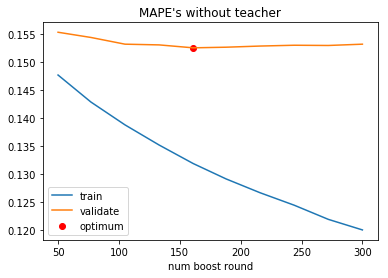
\includegraphics[width=10cm, height=6cm]
        {img/new0.png}}
      \end{figure}

\end{frame}


%-----------------------------------------------------------------------------------------------------
\begin{frame}{Использование привилегированной информации для смеси экспертов}
% \begin{block}{Использование обобщенной дистилляции}
% Варьируем параметр имитации, видим, что и сложность оптимальной модели, и ошибка, только растет.

\begin{figure}[!htb]
       \center{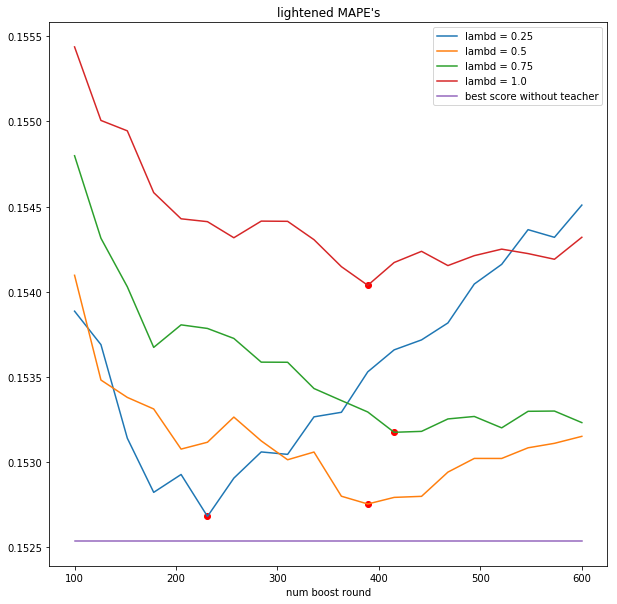
\includegraphics[width=7.5cm, height=7.5cm]
        {img/new1.png}}
\end{figure}

% \end{block}

\end{frame}

%-----------------------------------------------------------------------------------------------------
\begin{frame}{Использование привилегированной информации для смеси экспертов}
% \begin{block}{Использование обобщенной дистилляции}
% Варьируем параметр имитации, видим, что и сложность оптимальной модели, и ошибка, только растет.

\begin{figure}[!htb]
      \center{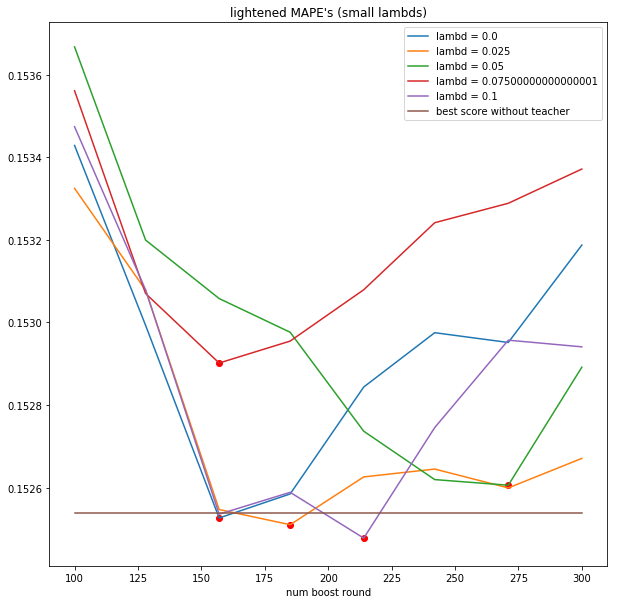
\includegraphics[width=7.5cm, height=7.5cm]
       {img/new2.png}}
\end{figure}

%\bigskip
%\centering{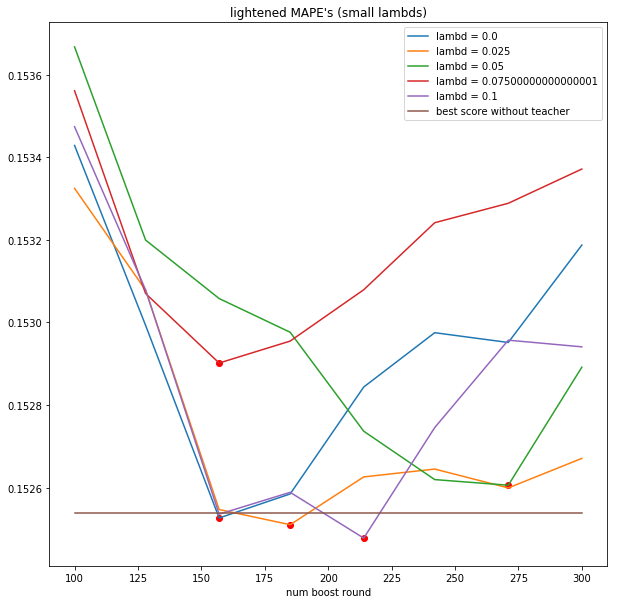
\includegraphics[width=250]{img/new2.png}}

% \end{block}

\end{frame}


%-----------------------------------------------------------------------------------------------------
\begin{frame}{Построение смеси экспертов}

Было взято несколько моделей, с различными степенями имитации, и числом итераций, оптимальным для них. В итоге алгоритм медленно сходится и дает большую ошибку:  MAPE = $19.6$ (против $15.3$ изначально). Веса показывают, что при большом модели с большим параметром имитации отбрасываются.   

\end{frame}

%-----------------------------------------------------------------------------------------------------
\begin{frame}{Дополнительный эксперимент}

Если брать не оптимальные модели учителя, а переобученные - качество оценки улучшается, но не значимо.

% \begin{block}{Использование обобщенной дистилляции}
% Варьируем параметр имитации, видим, что и сложность оптимальной модели, и ошибка, только растет.

\begin{figure}[!htb]
       \center{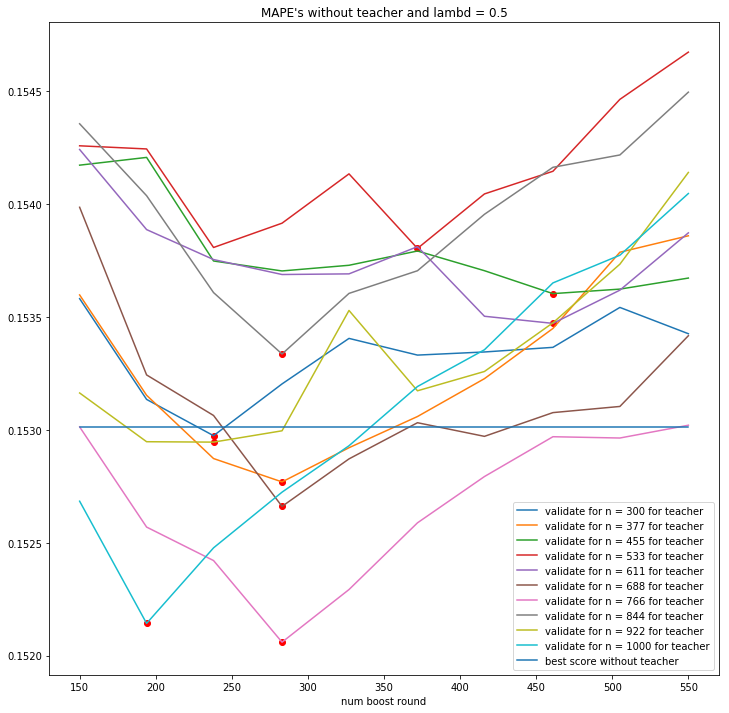
\includegraphics[width=7.5cm, height=7.5cm]
        {img/new4.png}}
\end{figure}

% \end{block}

\end{frame}

%-----------------------------------------------------------------------------------------------------
\begin{frame}{Результаты эксперимента}
\begin{block}{Основной эксперимент:}
Модели, построенные при помощи дистилляции, не только имеют худшее качество оценки, но ещё и  требуют большего числа ресурсов. Смесь экспертов, построенная на моделях с различным параметром дистилляции, также работает несколько хуже. 
Использование привилегированной информации не привело к положительному результату.
\end{block}

\begin{block}{Дополнительно:}
 Если в алгоритме дистилляции использовать не оптимальные параметры учителя, а параметры, дающие небольшое переобучение, результат становится лучше - но не значимо.
\end{block}

\end{frame}


%-----------------------------------------------------------------------------------------------------
\begin{frame}{Заключение}
\begin{block}{Выводы:}
\begin{itemize}
  \item Показан пример задачи машинного обучения, для которой дистилляция увеличивает вычислительную сложность алгоритма, но при этом качество оценки не улучшается.

  \item Зависимость качества оценки от параметра дистилляции немонотонно, и имеет локальные минимумы, которые находятся только экспериментальным путем.

\item Использование переобученного учителя в алгоритме дистилляции улучшает и качество оценки, и сложность модели

 \item Смесь экспертов - вычислительно сложный алгоритм, сходимость сильно от начальной иницилизации.

\end{itemize}
\end{block}
\end{frame}







\end{document} 